\documentclass{icthesis}

\usepackage{amssymb,amsmath,amsthm,array,epsfig,lmodern,pstricks,subfig,hyperref
,verbatim}

\newcommand{\R}{{\mathbb R}}
\newcommand{\vol}{\mathcal{L}^d}
\newcommand{\surfvol}{\mathcal{H}^{d-1}}
\newcommand{\dH}[1]{\;{\rm d}{\cal H}^{#1}} % Hausdorff measure
\newcommand{\dL}[1]{\;{\rm d}{\cal L}^{#1}} % Lebesgue measure
\newcommand{\bigchi}{\ensuremath{\mathrm{\mathcal{X}}}}
\newcommand{\charfcn}[1]{\bigchi_{#1}} % characteristic function
\newcommand{\Vh}{\underline{V}(\Gamma^m)}
\newcommand{\Wh}{W(\Gamma^m)}
\newcommand{\Vht}{\underline{V}(\Gamma^h(t))}
\newcommand{\Wht}{W(\Gamma^h(t))}
\newcommand{\uspace}{\mathbb{U}}
\newcommand{\pspace}{\mathbb{P}}
\newcommand{\kspace}{\mathbb{K}}
\newcommand{\xspace}{\mathbb{X}}
\newcommand{\sigmaO}{o}
\newcommand{\nabs}{\nabla_{\!s}}
\newcommand{\id}{\rm id}
\newcommand{\ddt}{\frac{\rm d}{{\rm d}t}}
\newcommand{\NbulkT}{\vec{N}_{\Gamma,\Omega}^T}
\newcommand{\Nbulk}{\vec{N}_{\Gamma,\Omega}}
\newcommand{\errorXx}{\|\Gamma^h - \Gamma\|_{L^\infty}}
\newcommand{\LerrorUu}[1]{\|\vec U - I^h_{#1}\,\vec u\|_{L^2}}
\newcommand{\HerrorUu}[1]{\|\vec U - I^h_{#1}\,\vec u\|_{H^1}}
\newcommand{\LerrorPp}{\|P - p\|_{L^2}}
\newcommand{\unitn}{\vec{\rm n}}
\newcommand{\mat}[1]{\underline{\underline{#1}}\rule{0pt}{0pt}}
\newcommand\Rey{\mbox{\textit{Re}}} %  Reynolds number

\begin{document}

\title{Front tracking finite element methods for two-phase Navier--Stokes flow}
\author{Marco Agnese}
\advisor{Robert N\"urnberg}
\degree{Doctor of Philosophy}
\field{Mathematics}
\degreeyear{2017}
\degreemonth{April}
\department{Mathematics}
%\pdOneName{B.Sc.}
%\pdOneSchool{Politecnico di Torino}
%\pdOneYear{2010}
%\pdTwoName{M.Sci.}
%\pdTwoSchool{Politecnico di Torino}
%\pdTwoYear{2013}

\maketitle
\setstretch{1.2}
\abstractpage
\dedicationpage
\acknowledgments
\listoffigures
\listoftables
\tableofcontents

\mainmatter
\setcounter{chapter}{-1}
\chapter{\sc Introduction}\label{ch:introduction}
Fluid flow problems with an unknown interface are ubiquitous in physics and
engineering. This introductory chapter is devoted to a description of the
mathematical model used to model this type of systems together with a brief
overview of the possible approaches to describe the unknown interface.

The chapter is organised as follows: in \S\ref{sec:free_boundary_flows}
we define what a free-boundary fluid flow is and we introduce a generic setting
for the problem; in \S\ref{sec:flow_equations} we present the
Navier--Stokes equations which govern the fluid; in
\S\ref{sec:bc_conditions} we discuss the boundary, initial and interface
conditions needed for the well possessedness of the problem; in
\S\ref{sec:interface_treatment} we briefly overview the different ways to
treat the unknown interface; in \S\ref{sec:numerical_challenges} we detail
the various numerical challenges posed by these types of flows; in
\S\ref{sec:numerical_implementation} we finally list the libraries used to
implement the numerical schemes described in this thesis and we provide the
links to the code developed in order to make all the results presented in this
work reproducible.

\section{Free-boundary fluid flows}\label{sec:free_boundary_flows}
Fluid flow problems with a moving interface are encountered in many
applications in physics, engineering and biophysics. Typical applications are
drops and bubbles, die swell, dam break, liquid storage tanks, dendritic growth,
ink-jet printing, fuel injection. For this reason, developing robust and
efficient numerical methods for these flows is an important problem and
has attracted tremendous interest over the last decade.

In these type of problems, apart from the flow solution in the bulk domain, the
position of a portion of the boundary is also unknown. This boundary can either
be an external boundary or an interface between sub-domains. At the
boundary/interface, certain boundary conditions need to be fulfilled, which
specify the position of the boundary. These conditions relate the variables of
the flow, velocity and pressure, across the domains under consideration of
external influences, such as for example surface tension. Numerically, in order
to be able to compute the flow solution as well as the boundary/interface
geometry, a measure to track the boundary starting from an initial position
needs to be incorporated.

The scenario we consider are two-phase flows, liquid-liquid or liquid-gas, in a
$d$-dimensional computational domain $\Omega\subset\R^d$. This domain
$\Omega$ contains two different immiscible fluids which, for all $t\in[0,T]$,
occupy time dependent regions $\Omega_+(t)$ and
$\Omega_-(t):=\Omega\setminus\overline{\Omega}_+(t)$ and
which are separated by an interface $(\Gamma(t))_{t\in[0,T]}$,
$\Gamma(t)\subset\Omega$. For later use, we always assume that
$(\Gamma(t))_{t\in [0,T]}$ is a sufficiently smooth evolving hypersurface
without boundary. See Figure~\ref{fig:two_phase_sketch} for an illustration.
\begin{figure}
\begin{center}
\unitlength15mm
\psset{unit=\unitlength,linewidth=1pt}
\begin{picture}(4,4)(0,0)
\psline(0,0)(4,0)(4,4)(0,4)(0,0)
\psline{->}(3,2)(3.5,2)
\pscustom[fillstyle=solid,fillcolor=lightgray!50]
{
\psellipse(2,2)(1,1)
}
\put(3.25,1.75){$\vec\nu$}
\put(1.75,0.75){{$\Gamma$}}
\put(1.75,2){{$\Omega_-$}}
\put(0.5,3.25){{$\Omega_+$}}
\end{picture}
\end{center}
\caption[Two-phase flow]{Two-phase flow setting.}
\label{fig:two_phase_sketch}
\end{figure}
Therefore both the sub-domains themselves and the flow field are part of the
solution. Indeed the main task in this context is to account for the interface
$\Gamma(t)$, which separates the distinct fluid domains and is generally in
motion. Apart from its exact position, the computation of geometrical quantities
of $\Gamma(t)$ such as its normal vector $\vec\nu$ and its mean curvature
$\varkappa$ are of interest.

\section{Flow governing equations}\label{sec:flow_equations}
For what concern the bulk flow, we restrict ourselves to isothermal conditions,
incompressible fluids and we assume that there is no change of phase. Under
this assumption, the fluid dynamics is modelled by the incompressible
Navier--Stokes equations. For more details see \cite{GrossR11}.

Denoting the velocity and pressure by $\vec u$ and $p$, respectively, we
introduce the Newtonian stress tensor
\begin{equation} \label{eq:stress_tensor}
\mat\sigma = \mu \,(\nabla\,\vec u + (\nabla\,\vec u)^T) - p\,\mat\id
= 2\,\mu\, \mat D(\vec u)-p\,\mat\id\,,
\end{equation}
where $\mu(t) = \mu_+\,\charfcn{\Omega_+(t)} + \mu_-\,\charfcn{\Omega_-(t)}$,
with $\mu_\pm \in \R_{>0}$, denoting the dynamic viscosities in the two phases,
$\mat\id \in \R^{d \times d}$ is the identity matrix and
$\mat D(\vec u):=\frac{1}{2}\, (\nabla\vec u+(\nabla\vec u)^T)$
is the rate-of-deformation tensor. Given a vector valued function $\vec
h:\R^d\to\R^d$, we define its gradient as
$\nabla\vec h = ((\nabla h_1)^T;\ldots;(\nabla h_d)^T)$. Moreover, let
$\rho(t) = \rho_+\,\charfcn{\Omega_+(t)} + \rho_-\,\charfcn{\Omega_-(t)}$,
with $\rho_\pm \in \R_{>0}$, be the fluid density.

Imposing the conservation of momentum and mass in each phase, the following
standard Navier--Stokes governing equations can be derived:
\begin{subequations}
\begin{alignat}{2}
\rho\,(\vec u_t +\vec u \,.\, \nabla \vec u)- \nabla\,.\,\mat\sigma
& = \vec f \quad &&\mbox{in } \Omega_\pm(t)\,,
\label{eq:ns_momentum} \\
\nabla\,.\,\vec u & = 0 \quad &&\mbox{in } \Omega_\pm(t)\,,
\label{eq:ns_mass}
\end{alignat}
\end{subequations}
where $\vec f$ includes all external body forces referred to the unit mass of
fluid.

Substituting (\ref{eq:stress_tensor}) in (\ref{eq:ns_momentum}), we obtain the
well known incompressible Navier--Stokes model:
\begin{subequations}
\begin{alignat}{2}
\rho\,(\vec u_t +\vec u \,.\, \nabla \vec u) -2 \mu\,\nabla\,.\,\mat D(\vec u)+
\nabla\,p & = \vec f \quad &&\mbox{in } \Omega_\pm(t)\,,
\label{eq:ns_momentum_bis} \\
\nabla\,.\,\vec u & = 0 \quad &&\mbox{in } \Omega_\pm(t)\,.
\label{eq:ns_mass_bis}
\end{alignat}
\end{subequations}

To better grasp the physical meaning of the terms appearing in the momentum
equation (\ref{eq:ns_momentum_bis}) we briefly describe them. The inertia term
$\vec u \,.\, \nabla \vec u$ is a convection term arising from the conservation
of momentum. The momentum of each portion of fluid needs to be conserved
therefore it needs to move with the fluid which means that it is convected with
the fluid. The pressure term $\nabla\,p$  is originated by the Newtonian
constitutive equation (\ref{eq:stress_tensor}) and it represent all the forces
resulting from pressure differences within the fluid. Finally, the friction
term $\nabla\,.\,\mat D(\vec u)$, which again arises from the Newtonian
constitutive equation (\ref{eq:stress_tensor}), is a diffusion operator
equalizing the velocity of neighbouring elements. The more viscous the fluid,
the stronger is the friction between neighbouring particles and thus the
equalizing effect.

The Reynolds number $\Rey$ is an important dimensionless quantity in fluid
mechanics and it is defined as
\begin{equation}\label{eq:reynolds}
\Rey=\frac{\rho\,u_c\,L_c}{\mu}\,,
\end{equation}
where $L_c$ is the characteristic dimension of the problem and $u_c$ is the
characteristic velocity of the fluid. It quantifies the ratio of inertial
forces to viscous forces within the fluid, therefore it is used to predict
flow patterns in different fluid flow situations. If $\Rey \ll 1$ the flow is
laminar due to the fact that viscous forces are dominant and it is
characterized by smooth, constant fluid motion.  Otherwise, the flow is
turbulent due to the fact that inertial forces are dominant and it tends to
produce chaotic eddies, vortices and other flow instabilities.

In the case of laminar flow, the advective term in the momentum equation
(\ref{eq:ns_momentum}) can be neglected, giving rise to the so called Stokes
equations
\begin{subequations}
\begin{alignat}{2}
- \nabla\,.\,\mat\sigma & = \vec f \quad &&\mbox{in } \Omega_\pm(t)\,,
\label{eq:momentum} \\
\nabla\,.\,\vec u & = 0 \quad &&\mbox{in } \Omega_\pm(t)\,,
\label{eq:mass}
\end{alignat}
\end{subequations}
which for Newtonian fluids are expressed as
\begin{subequations}
\begin{alignat}{2}
-2 \mu\,\nabla\,.\,\mat D(\vec u)+ \nabla\,p & = \vec f \quad &&\mbox{in }
\Omega_\pm(t)\,,
\label{eq:momentum_bis} \\
\nabla\,.\,\vec u & = 0 \quad &&\mbox{in } \Omega_\pm(t)\,.
\label{eq:mass_bis}
\end{alignat}
\end{subequations}

We finally observe that for the one-phase Navier--Stokes flow,
$\rho_+=\rho_-=\rho$ and $\mu_+=\mu_-=\mu$, using the
incompressibility condition (\ref{eq:ns_mass_bis}) we have
\begin{equation}
2\nabla\,.\,\mat D(\vec u) = \nabla\,.\big(\nabla\vec u+(\nabla\vec u)^T\big)=
\Delta \vec u + \nabla(\nabla\,.\vec u) = \Delta \vec u
\end{equation}
therefore the system (\ref{eq:ns_momentum_bis}--b) can be rewritten as
\begin{subequations}
\begin{alignat}{2}
\rho\,(\vec u_t +\vec u \,.\, \nabla \vec u) - \mu\,\Delta\vec u+\nabla\,p
& = \vec f \quad \mbox{in } \Omega\,, \\
\nabla\,.\,\vec u & = 0 \quad \mbox{in } \Omega\,,
\end{alignat}
\end{subequations}
which is the canonical form of the one-phase Navier--Stokes problem.

\section{Boundary, initial, and interface conditions}\label{sec:bc_conditions}
For the full Navier--Stokes problem (\ref{eq:ns_momentum_bis}-b), a
divergence-free velocity field for the whole computational domain is needed as
an initial condition. Therefore we impose
\begin{equation}\label{eq:ns_ic}
\vec u(0) = \vec u_0 \quad \mbox{in } \Omega\,.
\end{equation}
The initial condition is not need in the Stokes case (\ref{eq:momentum_bis}-b)
since it is a stationary problem.

In order to obtain a well-posed system, boundary conditions have to be imposed
on the bulk domain boundary $\partial\Omega$. Let $\partial\Omega$ be
partitioned as $\partial\Omega=\partial_1\Omega \cup \partial_2\Omega$ with
$\partial_1\Omega \cap \partial_2\Omega = \emptyset$. We use the Dirichlet
condition on $\partial_1 \Omega$
\begin{equation}\label{eq:ns_bc_dirichlet}
\vec u = \vec g \quad \mbox{on } \partial_1 \Omega\,,
\end{equation}
and the free-slip condition on $\partial_2 \Omega$
\begin{equation}\label{eq:ns_bc_freeslip}
\vec u \,.\,\unitn = 0  \quad \mbox{on } \partial_2 \Omega\,,
\end{equation}
with $\unitn$ denoting the outer unit normal of $\partial \Omega$. We notice
that the case $\vec g = \vec 0$ corresponds to the so called no-slip condition.

Since we are dealing with a two-phase flow, some interface conditions are also
needed on the unknown interface $\Gamma(t)$, which couple the velocity and
stress between the two domains. Viscosity of the fluids leads to the continuity
condition
\begin{equation}\label{eq:interface_jump_velocity}
[\vec u]_-^+ = \vec 0 \quad \mbox{on } \Gamma(t)\,,
\end{equation}
where $[\vec u]_-^+ := \vec u_+ - \vec u_-$ denote the jump in velocity across
the interface $\Gamma(t)$. Here and throughout, we employ the shorthand notation
$\vec h_\pm := \vec h\!\mid_{\Omega_\pm(t)}$ for a function
$\vec h : \Omega \times [0,T] \to \R^d$; and similarly for scalar and
matrix-valued functions.

The assumption that there is no change of phase leads to the dynamic interface
condition
\begin{equation}\label{eq:interface_velocity}
\V\,.\,\vec\nu = \vec u\,.\,\vec \nu \quad \mbox{on }
\Gamma(t)\,,
\end{equation}
given that $\V$ is the velocity of the evolving interface
$\Gamma(t)$ and where $\vec\nu(t)$ is the unit normal on $\Gamma(t)$ pointing
into $\Omega_+(t)$. Therefore the normal velocity of the interface needs to
match the flow normal velocity across the interface $\Gamma(t)$.

The momentum conservation in a small material volume that intersects the
interface leads to the stress balance condition
\begin{equation}\label{eq:interface_jump_stress_div}
[\mat\sigma\,\vec \nu]_-^+ = -\nabs\,.\mat\sigma_{\Gamma} \quad \mbox{on }
\Gamma(t)\,,
\end{equation}
where $\mat\sigma_{\Gamma}$ is the interface stress tensor and $\nabs\,.$ is
the surface divergence on $\Gamma(t)$. The operator $\nabs$ is the surface
gradient on $\Gamma(t)$ and it is the orthogonal projection of the usual
gradient operator $\nabla$ on the tangent space of the surface $\Gamma(t)$.
Therefore, given a smooth function $h$ defined on a neighbourhood of
$\Gamma(t)$, it is defined as
\begin{equation}\label{eq:surface_gradient}
\nabs\,h(\vec z)=\mat P\,\nabla\,h(\vec z)=\nabla\,h(\vec z)\,-
\,\nabla\,h(\vec z)\,.\,\vec\nu(\vec z)\,\vec\nu(\vec z)\,,\quad \vec z
\in\Gamma(t)\,,
\end{equation}
with the usual projection operator $\mat P$ defined as
\begin{equation}\label{eq:surface_projection}
\mat P(\vec z)=\mat\id\,-\,\vec\nu(\vec z)\,\vec\nu(\vec z)^T\,,\quad \vec
z\in \Gamma(t)\,.
\end{equation}
It can be shown that the definition of $\nabs\,h$ does not depend on the chosen
extension of $h$, but only on the value of $h$ on $\Gamma(t)$. See
\cite{DeckelnickDE05}. For later use, we also define the surface Laplacian, also
known as Laplace--Beltrami operator, $\Delta_s$ on $\Gamma(t)$ as
\begin{equation}\label{eq:surface_laplacian}
\Delta_s = \nabs\,.\,\nabs\,.
\end{equation}

We restrict ourselves to the case that the only force acting on the interface
is the surface tension contact force. Therefore the interface stress tensor
$\mat\sigma_\Gamma$ has the following constitutive equation
\begin{equation}\label{eq:interface_stress_tensor}
\mat\sigma_{\Gamma}=\gamma\,\mat P\,,
\end{equation}
where $\gamma$ is the surface tension coefficient. Substituting
(\ref{eq:interface_stress_tensor}) in (\ref{eq:interface_jump_stress_div}) we
obtain
\begin{equation}\label{eq:interface_stress_tensor_divergence}
\begin{align*}
[\mat\sigma\,\vec \nu]_-^+ &= -\nabs\,.(\gamma\,\mat P)
= -\gamma\,\nabs\,.\,\mat P-\nabs\,\gamma
= \gamma\nabs\,.\,(\vec\nu\,\vec\nu^T)-\nabs\,\gamma \\
& = \gamma\nabs\,.\,\vec\nu\,\vec\nu + \gamma\nabs\,\vec\nu\,.\,\vec\nu
- \nabs\,\gamma = \gamma\nabs\,.\,\vec\nu\,\vec\nu - \nabs\,\gamma \\
& = -\gamma\,\varkappa\,\vec\nu - \nabs\,\gamma \quad \mbox{on } \Gamma(t)\,,
\end{align*}
\end{equation}
where we have used the fact that the surface gradient $\nabs$ is, by definition,
always orthogonal to the surface normal $\vec\nu$ and that $\varkappa =
-\nabs\,.\vec\nu$ is the mean curvature of $\Gamma(t)$. The projection $\mat P$
is used, since $\mat\sigma_{\Gamma}$ should represent only contact forces that
are tangential to the surface. We assume that $\gamma$ is constant and
therefore, from (\ref{eq:interface_stress_tensor_divergence}), we obtain the
so called clean interface model for the interfacial forces
\begin{equation}\label{eq:interface_jump_stress}
[\mat\sigma\,\vec \nu]_-^+ = -\gamma\,\varkappa\,\vec\nu \quad \mbox{on }
\Gamma(t)\,.
\end{equation}

Finally, in order to have a well-posed problem, one needs suitable initial
conditions for the interface. Therefore we set $\Gamma(0)=\Gamma_0$.

\section{Interface treatment}\label{sec:interface_treatment}
The dynamics of the interface are determined by the condition
(\ref{eq:interface_velocity}) which, however, describes the dynamics in a
strongly implicit way since the velocity field $\vec u$ depends on the
position of the interface itself. In numerical simulations, there are
several strategies to deal with this problem, which can be divided into two
categories depending on the viewpoint: interface capturing and interface
tracking.

Interface capturing methods use an Eulerian description of the interface, which
is defined implicitly. A characteristic scalar field $\psi$ is used to identify
the two phases as well as the interface along the boundaries of the individual
fluid domains. Depending on the method, this scalar field may be, for example,
a discontinuous Heaviside function or a signed-distance function. The interface
motion is taken into account using a standard advection equation
\begin{equation}
\frac{\partial \psi}{\partial t}+\vec u\,.\nabla\,\psi=0 \quad \mbox{in }
\Omega\,,
\end{equation}
which transports the scalar field with the fluid velocity $\vec u$. The most
important methods, which belong to this this category, are the particle method,
the volume-of-fluid method, the level-set method and the phase-field method.
The particle method utilizes mass-less particles distributed in an Eulerian
mesh to capture the fluid flow and in particular the interface position, see
e.g \cite{Girault1976}. In the volume-of-fluid method, the characteristic
function of one of the phases is approximated numerically, see e.g.
\cite{HirtN81,RenardyR02,Popinet09}. In the level-set method, the interface is
given as the level set of a function, which has to be determined, see e.g.
\cite{SussmanSO94,Sethian99,OsherF03,GrossR07}. Instead, the phase-field method
works with diffuse interfaces, and therefore the transition layer between the
phases has a finite size. There is no tracking mechanism for the interface, but
the phase state is included implicitly in the governing equations. The
interface is associated with a smooth, but highly localized variation of the
so-called phase-field variable. We refer to
\cite{HohenbergH77,AndersonMW98,LowengrubT98,Feng06,KaySW08,AbelsGG12,GrunK14}
for details. In general, the great advantage of the interface capturing
approaches is that they are inherently able to deal with topological changes of
the interface. This allows a much more flexible interface description than in
interface tracking approaches. On the other hand, it is challenging to treat
accurately discontinuous quantities across the interface, to have mass
conservation within each phase and to apply boundary conditions along the
interface.

Interface tracking approaches, instead, use a Lagrangian description of the
interface which is described explicitly. The idea is to take a (virtual)
particle on the interface at time $t=t_0$ with Eulerian coordinates $\vec z(0)
\in \Gamma_0$. Let $\vec z(t)$ be the Eulerian coordinates of this particle,
with $t\geq t_0$. The particles on the interface are transported by the flow
velocity $\vec u$, therefore it holds the equation
\begin{equation}
\frac{\partial \vec z(t)}{\partial t}=\vec u(\vec z(t),t)\,,
\end{equation}
which determines the path of a material particle and consequently it
characterizes the evolution of the interface. This interface representation
forms the basis of the interface tracking methods. In these methods a
collection of markers is put on a given interface $\Gamma_0$ and then
transported (numerically) by the flow velocity $\vec u$ to obtain the markers
on the interface $\Gamma(t)$. Usually, the collection of markers on $\Gamma_0$
are the set of vertices of the triangulation of $\Gamma_0$. The great
advantage of interface tracking approaches is that they offer an accurate and
computationally efficient approximation of the evolving interface. Moreover,
the imposition of boundary conditions at the interface is simple since the mesh
nodes lies on the interface itself. However, firstly the mesh quality will
usually degrade quickly in the case of large deformations and secondly
topological changes require a special treatment. In order to keep an
acceptable mesh quality throughout the simulation, mesh smoothing techniques
are applied and, when they are not enough, a full remeshing is used. If
topological changes occur, the only way to tackle the issue is to
perform a remeshing with respect to the new interface. The main consequence of
remeshing is the need to project the field values from the old to the new
mesh, a ceaseless source for errors, and at the same time computationally
costly especially in dimension 3. Therefore, it is desirable to keep the
frequency of remeshing as low as possible. We refer e.g. to
\cite{UnverdiT92,Bansch01,Tryggvason_etal01,GanesanMT07,GanesanT08,spurious}
for further details, and to \cite{LevequeL97,Peskin02} for the related immersed
boundary method, which is used to simulate fluid-structure interactions using
Eulerian coordinates for the fluid and Lagrangian coordinates for the structure.

In the following chapters, we always use an interface tracking approach to
describe the interface evolution. In particular, we adopt a fitted mesh approach
which means that the discrete interface is composed by bulk element faces.
Consequently there is a strong coupling between the bulk mesh and the interface
mesh.

\section{Numerical challenges}\label{sec:numerical_challenges}
Two-phase flows pose enormous challenges to numerical simulation tools and
they can not be solved reliably and accurately by the commercial software that
are available nowadays. Therefore, compared to one-phase flow solvers, special
tailor-made numerical schemes have to be developed. Below we address some causes
of the very high numerical complexity of this problem class.

The evolution of the unknown interface is determined by the simple dynamic
condition (\ref{eq:interface_velocity}). Unfortunately, it turns out that an
accurate numerical approximation of the geometric object representing the
interface and its evolution is a very difficult task. This task become even
more complicated in cases of geometric singularities such as droplet break up or
collision. Although several techniques have been developed, an accurate
interface approximation remains a challenging task.

For high Reynolds number, the flow model is strongly nonlinear. Therefore the
coupling between fluid dynamics and interface evolution turns out to be strongly
nonlinear. This nonlinearity cause difficulties for the construction of
accurate numerical schemes for time discretization.

Usually several quantities are discontinuous across the interface. Indeed, for
example, the value of density and viscosity have jumps across the interface,
since the interface separates two different fluids. Moreover, due to surface
tension forces, also the pressure is discontinuous across the interface. In
most applications the stress balance (\ref{eq:interface_jump_stress_div}) and a
jump in the viscosity across the interface typically induce a discontinuity
across the interface of the normal derivative of the velocity. Of particular
importance is the precise inclusion of surface tension terms, and the correct
handling of discontinuity jumps in the material properties and in the pressure
at the interface, in order to suppress spurious velocities, which are also
called parasitic currents. Apart from stationary problems, the unknown
interface is changing as a function of time and therefore these discontinuities
are moving. The numerical treatment of moving discontinuities often causes
severe difficulties.

The full discretization in space and in time results in a very large nonlinear
system of equations at each time step. Most of the total computing time is
spent solving these large nonlinear systems and therefore it is crucial to use
efficient iterative solvers. The efficiency can be largely improved by using
special techniques that are adapted to the problem class, in the sense that the
solver makes use of certain structural properties of the problem.

\section{Numerical implementation}\label{sec:numerical_implementation}
We implement all numerical schemes from scratch in \verb|C++| within the
\verb|DUNE| framework, see \cite{dunegridpaperI08,dunegridpaperII08}.
\verb|DUNE|, the Distributed and Unified Numerics Environment is a modular and
extensible toolbox for solving partial differential equations with grid-based
methods. It supports different schemes based on finite elements, finite volumes
and finite differences. We use the following \verb|DUNE| modules:
\verb|dune-common| (build system, infrastructure and foundation classes),
\verb|dune-istl| (algebraic solvers), \verb|dune-geometry| (geometric
entities), \verb|dune-grid| (grid manager interface) and \verb|dune-fem| (FEM
toolbox), see \cite{dunefempaper10}. More information on the library can be
found on the official website \myurl{https://www.dune-project.org/}.

We actively contributed to the various modules of the library providing
upstream patches for new features and bug fixing with more than $4\cdot 10^4$
lines of changes.

As grid manager we use \verb|ALBERTA|, see \cite{Alberta}, available here
\myurl{http://www.alberta-fem.de/}. We also use the sparse factorization
package \verb|SuiteSparse|, see \cite{Davis04}, available here
\myurl{http://faculty.cse.tamu.edu/davis/suitesparse.html}.

We implement the scheme described in Chapter \ref{ch:geometric_pdes} as a
\verb|DUNE| module named \verb|dune-geometric-pde|, available here
\myurl{https://github.com/magnese/dune-geometric-pde}, while the schemes
described in Chapter \ref{ch:stokes} and Chapter \ref{ch:navier_stokes}
are implemented as a \verb|DUNE| module called
\verb|dune-navier-stokes-two-phase|, available here
\myurl{https://github.com/magnese/dune-navier-stokes-two-phase}.

All the meshes are created with the library \verb|Gmsh|, see
\cite{GeuzaineR09}, available here \myurl{http://gmsh.info/} and the plots are
generated with either \verb|ParaView|, available here
\myurl{http://www.paraview.org/}, or \verb|Gnuplot|, available here
\myurl{http://www.gnuplot.info/}.

All the simulations we report on are performed on a Linux cluster equipped with
\verb|Ubuntu 14.04.1 LTS| and compiled with \verb|g++ 5.3.0|. The cluster is
heterogeneous and consist of 32 computing nodes. Each node is equipped
with dual Xeon CPUs containing either 4 or 6 processor cores with frequency
ranging from 2.40GHz to 3.00GHz and memory between 16GB and 48GB. The CPU times
are measured in seconds and correspond to the wall time of a single thread
computation.
\chapter{\sc Geometric Evolution Equations}
\label{ch:1}

\section[Geometric PDEs]{Geometric PDEs}
As starting point, in order to describe the key ideas of the front tracking
approach, we consider the simple problem of purely geometric evolution
equations. A geometric evolution equation defines the motion of a hypersurface
by prescribing its normal velocity in terms of its geometric quantities. These
problems are part of the more general time-dependent interface evolution
problems category, where the normal velocity depends also on field quantities
evaluated on the analysed hypersurface. A detailed description and analysis can
be found in the review article \cite{DeckelnickDE05}.

Interface evolution problems are everywhere in modern physics and engineering.
Several typical applications can be found in materials science such as the
mathematical modelling of the morphology of microstructure in order to
correctly evaluate the mechanical properties of the material or in void
electro-stress migration where small voids or cracks contained in metallic
materials can change their location and shape according to the presence of
surface diffusion and electro-stress loading. Other typical applications which
can be modelled as time-dependent interface evolution problems are the motion of
grain boundaries which separate differing orientations of the same crystalline
phase, or solid-liquid interfaces exhibiting dendritic structures in
under-cooled solidification. Another research fields where these models can be
applied is image processing to detect the separation of dark regions from a
brighter background and to identify separating contours in order to correctly
cluster the objects in the image. Instead, as explained in Chapter
\ref{ch:introduction}, we apply these techniques to incompressible two-phase
flows problem.

A general geometric evolution equation has the following formulation
\begin{equation}\label{eq:geometric_pde}
\vec{\mathcal{V}}\,.\,\vec\nu=f(\vec{z}\,,\vec{\nu}\,,\varkappa)
\qquad\mbox{on }\Gamma(t),
\end{equation}
which prescribes the normal velocity $\vec{\mathcal{V}}\,.\,\vec\nu$ of the
interface $\Gamma(t)$ as a function depending on the position $\vec z$, its
normal direction $\vec{\nu}$ and the sum of its principal curvatures
$\varkappa$. The evolution equation (\ref{eq:geometric_pde}) prescribes only
the normal velocity therefore the overall goal is to find a family of
solutions $\{ \Gamma(t) \}_{t \in [0, T]}$ of closed compact and orientable
hypersurfaces in $\R^{d}$ ($d = 2$ for curves, $d = 3$ for surfaces).

The simplest geometric PDE is the one which arises from motion by mean
curvature,
\begin{equation}\label{eq:mean_curvature}
\vec{\mathcal{V}}\,.\,\vec\nu=\varkappa\qquad\mbox{on }\Gamma(t).
\end{equation}
This equation describes a surface evolving in such a way that its own normal
velocity is equal to the sum of the $d-1$ principal curvatures of $\Gamma(t)$.

Another important geometric PDE is the one which arises from motion by
surface diffusion
\begin{equation}\label{eq:surface_diff}
\vec{\mathcal{V}}\,.\,\vec\nu=-\Delta_s \varkappa \qquad\mbox{on }\Gamma(t)\,,
\end{equation}
where we use the Laplace--Beltrami operator $\Delta_s$ defined by
(\ref{eq:surface_laplacian}). In this case the surface normal velocity matches
the surface Laplacian of the mean curvature.

For both models, (\ref{eq:mean_curvature}) and (\ref{eq:surface_diff}), it is
necessary to prescribe the initial interface $\Gamma(0)=\Gamma_0$ in order to
have a well posed problem.

\section[Geometric Analysis]{Geometric analysis}
The aim of this section is to collect some useful definitions and results from
differential geometry. Again we refer to \cite{DeckelnickDE05} which cover the
subject in depth.

A subset $\Gamma \subset \R^d$ is called a $C^2$-hypersurface if for each point
$\vec z_0 \in \Gamma$ there exists an open set $G \subset \R^d$ containing
$\vec z_0$ and a function $g \in C^2(G)$ such that
\begin{equation}
G \cap \Gamma = \{ \vec z \in G \, | \, g(\vec z) = 0 \}
\qquad \mbox{ and } \qquad \nabla \, G(\vec z) \neq 0\,,
\quad \forall\ \vec z \in G \cap \Gamma \, .
\end{equation}
The tangent space $T_{\vec z} \Gamma$ is then the $(d-1)$-dimensional linear
subspace of $\R^d$ that is orthogonal to $\nabla \, g(\vec z)$. It does not
depend on the particular function $g$ which is chosen to describe $\Gamma$. A
$C^2$-hypersurface $\Gamma \in \R^d$ is called orientable if there exists a
vector-valued function $\vec\nu \in C^1(\Gamma, \R^d)$, i.e.~$\vec\nu \in C^1$
in an open neighbourhood of $\Gamma$, such that $\vec\nu(\vec z) \perp T_{\vec
z} \Gamma$ and $|\vec{\nu}(\vec z)| = 1$ for all $\vec z \in \Gamma$. In what
follows, we shall assume that $\Gamma \subset \R^d$ is an orientable
$C^2$-hypersurface.

In order to prove some property of the surface gradient
(\ref{eq:surface_gradient}), we employ the notation
\begin{equation}
\nabla_s \, g(\vec z) = (\underline{D}_1 g(\vec z), \hdots, \underline{D}_{d}
g(\vec z))
\end{equation}
for the $d$ components of the surface gradient. Since $\nabla_s \, g(\vec z)$
is the orthogonal projection of $\nabla \, g(\vec z)$ onto $T_{\vec z} \Gamma$,
it depends only on the values of $g$ on $\Gamma$. Moreover, from
(\ref{eq:surface_gradient}) follows that
\begin{equation}\label{eq:surface_gradient_comp}
\nabla_s \, g(\vec z) \,.\, \vec{\nu}(\vec z)=0\,, \qquad \vec z \in \Gamma\,.
\end{equation}
Similarly, if $g$ is twice differentiable in an open neighbourhood of
$\Gamma$, the surface Laplacian (\ref{eq:surface_laplacian}) can be written as
\begin{equation}\label{eq:surface_laplacian_comp}
\Delta_s g(\vec z) = \nabla_s\, . \,\nabla_s \, g(\vec z) =
\sum_{i = 1}^d \underline{D}_i \underline{D}_i g(\vec z) \, ,
\qquad \vec z \in \Gamma \, ,
\end{equation}
while, if $\vec g$ is a differentiable vector field, the surface divergence
can be rewritten as
\begin{equation}
\nabla_s \,.\, \vec g(\vec z) = \sum_{j = 1}^{d} \underline{D}_j \vec g_j
(\vec z)\,, \qquad \vec z \in \Gamma\,.
\end{equation}

We assume $\vec{\nu} \in C^1$ in a neighbourhood of $\Gamma$ so that we
may introduce the matrix $\mat H(\vec z)$ with components
\begin{equation}\label{eq:matrixHjk}
[\mat H (\vec z)]_{jk} = - \underline{D}_j \nu_k (\vec z)\,, \qquad \vec z \in
\Gamma \, ,
\end{equation}
with $1\leq j,k\leq n$. It can be shown that $\mat H(\vec z)$ is symmetric.
Furthermore,
\begin{equation}
\sum_{k = 1}^{d} [\mat H(\vec z)]_{jk} \nu_k (\vec z) =
\sum_{k = 1}^{d} - \underline{D}_j \nu_k (\vec z) \nu_k (\vec z) =
- \tfrac{1}{2} \underline{D}_j |\vec{\nu}|^2 (\vec z) = 0 \, ,
\end{equation}
since $|\vec{\nu}| = 1$ on $\Gamma$. Thus, $\mat H(\vec z)$ has one
eigenvalue which is equal to zero with corresponding eigenvector
$\vec\nu(\vec z)$. The remaining $d - 1$ eigenvalues $\varkappa_1 (\vec z),
\hdots, \varkappa_{d - 1} (\vec z)$ are called the principal curvatures of
$\Gamma$ at the point $\vec z$. The mean curvature of $\Gamma$ at $\vec z$
can then be defined as the trace of the matrix $\mat H(\vec z)$, that is
\begin{equation}\label{eq:definitionMC}
\varkappa (\vec z) = \sum_{j = 1}^{d} [\mat H(\vec z)]_{jj} = \sum_{j = 1}^{d -
1} \varkappa_j (\vec z) \,.
\end{equation}
Note that (\ref{eq:definitionMC}) differs from the more common
definition of mean curvature,
$\varkappa = \frac{1}{d - 1} \sum_{j = 1}^{d - 1} \varkappa_j$.
From (\ref{eq:matrixHjk}) we derive the following expression for mean
curvature:
\begin{equation}\label{eq:definition2MC}
\varkappa (\vec z)=-\nabla_s \,.\, \vec{\nu}(\vec z) \qquad \vec z \in \Gamma\,.
\end{equation}
In particular, if $\Gamma$ is the unite sphere,
$\Gamma = \{ \vec z \in \R^d : |\vec z| = 1 \}$,
and the unit normal field is chosen to point away from $\Gamma$,
i.e.~$\vec\nu(\vec z) = \vec z$, we obtain that $\varkappa = -
(d - 1)$, on considering the particular function $g(\vec z) = z_j$, $j \in \{
1, \hdots, d \}$ and observing that $\underline{D}_i z_j = \delta_{ij} - \nu_j
\nu_i$. This shows that the mean curvature $\varkappa$ is positive if $\Gamma$
is curved in the direction of the normal.

Moreover, while the sign of $\varkappa$ depends on the choice of the normal
$\vec\nu$, the mean curvature vector $\varkappa \vec\nu$ is an invariant. By
choosing again the particular function $g(\vec z) = z_j$, $j \in \{ 1,
\hdots, d \}$ in (\ref{eq:surface_laplacian_comp}) and recalling the application
of the Laplace-Beltrami operator to each independent variable $z_j$, we deduce
that
\begin{equation}
\Delta_s z_j = - \sum_{i = 1}^{d} \underline{D}_i (\nu_j \nu_i) =
- (\nabla_s \,.\, \vec\nu) \nu_j - \nabla_s \, \nu_j \,.\, \vec\nu = \varkappa
\nu_j\, ,
\end{equation}
which leads to the identity
\begin{equation} \label{eq:LBop}
\Delta_s\, \vec \id = \varkappa\, \vec\nu \qquad \mbox{on $\Gamma(t)$}\,.
\end{equation}
This identity of differential geometry will be useful at a later stage to
obtain a weak formulation of the surface diffusion and mean curvature problems.

\section[Properties of geometric flows]{Properties of geometric flows}
Here we report some fundamental properties of the mean curvature flow and
surface diffusion. In order to derive these properties, we need a transport
theorem for integrals. Consider a family $\{ \Gamma(t) \}_{t \in [0, T]}$
of hypersurfaces that evolve over time. Such a family is called a
$C^{2,1}$-family of hypersurfaces if, for each point $(\vec z_0, t_0) \in
\R^{d} \times (0, T)$ with $\vec z_0 \in \Gamma_0$, there exists an
open set $G \subset \R^{d}$, $\delta > 0$ and a function
$g \in C^{2,1}(G \times (t_0 - \delta, t_0 + \delta))$ such that
\begin{equation}
G \cap \Gamma (t) = \{ \vec{z} \in G \, | \, g (\vec z, t) = 0 \}
\qquad \mbox{ and } \qquad \nabla \, g (\vec z, t) \neq 0
\quad \forall\ \vec z \in G \cap \Gamma(t) \, .
\end{equation}

Now take a family $\{ \Gamma(t) \}_{t \in [0, T]}$ of evolving hypersurfaces
which satisfies the above assumptions and, moreover, suppose that each surface
$\Gamma(t)$ is compact. We are interested in the time derivative of certain
volume and area integrals. As usual, $\surfvol$ is the $(d-1)$-dimensional
Hausdorff measure and $\vol$ is the Lebesgue measure in $\R^d$.

\begin{lemma}
Let $g \in C^1(Q)$, where $Q$ is an open set containing

\begin{equation}
\bigcup_{0 < t < T} \Gamma(t) \times \{ t \} \, .
\end{equation}

Suppose in addition that each surface $\Gamma(t)$ is the boundary of an open
bounded subset $\Omega(t) \subset \R^{d}$. Then

\begin{align}
\ddt \int_{\Omega(t)} g \, \dL{d} & =
\int_{\Omega(t)} \frac{\partial g}{\partial t} \, \dL{d}
+ \int_{\Gamma(t)} g \,\vec{\mathcal{V}}\,.\,\vec\nu \, \dH{d-1} \, ,
\label{eq:variationVolume} \\
\ddt \int_{\Gamma(t)} g \, \dH{d-1} & =
\int_{\Gamma(t)} \frac{\partial g}{\partial t} \, \dH{d-1} -
\int_{\Gamma(t)} g \, \vec{\mathcal{V}}\,.\,\vec\nu \varkappa \, \dH{d-1}
\nonumber \\
& + \int_{\Gamma(t)} \frac{\partial g}{\partial \vec{\nu}}\,
\vec{\mathcal{V}}\,.\,\vec\nu \, \dH{d-1} \, .
\label{eq:variationLength}
\end{align}
\end{lemma}

\begin{proof}
For a proof, see \cite[\S~2.6, Lemma 2.1]{DeckelnickDE05}.
\end{proof}

The evolution of an hypersurface subject to the mean curvature flow
(\ref{eq:mean_curvature}) exhibits the interesting area-decreasing property,
which is obtained from the following lemma.

\begin{lemma}
Let $\Gamma(t)$ be a family of evolving hypersurfaces
satisfying \eqref{eq:mean_curvature} and assume that each $\Gamma(t)$ is
compact. Then

\begin{equation}
\int_{\Gamma(t)} (\vec{\mathcal{V}}\,.\,\vec\nu)^2 \, \dH{d-1} +
\ddt \surfvol(\Gamma(t)) = 0 \, . \label{eq:lengthDecrease}
\end{equation}

\end{lemma}

\begin{proof}
Choosing $g \equiv 1$ in (\ref{eq:variationLength}) and the evolution law
(\ref{eq:mean_curvature}) yields the desired result.
\end{proof}
The case $d = 2$ is usually referred to as curve shortening flow.

On the other hand, the evolution of an hypersurface subject to surface
diffusion (\ref{eq:surface_diff}) conserves, for closed hypersurfaces, the
enclosed volume and decreases the area as obtained from the following
lemma

\begin{lemma}
Let $\Gamma(t)$ be a family of evolving hypersurfaces
satisfying \eqref{eq:surface_diff} and assume that each $\Gamma(t)$ is
compact and closed. Then
\begin{align}
\ddt \vol(\Omega(t)) & = 0 \,, \label{eq:conservationVolume} \\
\ddt \surfvol (\Gamma(t)) & \leq 0 \,.\label{eq:areaDecrease}
\end{align}
\end{lemma}

\begin{proof}
For (\ref{eq:conservationVolume}), choosing $g \equiv 1$ in
(\ref{eq:variationVolume}) and the evolution law (\ref{eq:surface_diff}) yields
to
\begin{align*}
\ddt \vol(\Omega(t)) &= - \int_{\Gamma(t)} \vec{\mathcal{V}}\,.\,\vec\nu \,
\dH{d-1} = \nonumber \\
\int_{\Gamma(t)} \Delta_s \, \varkappa \, \dH{d-1} &= - \int_{\Gamma(t)}
\nabla_s \, \varkappa \,.\, \nabla_s \, 1 \, \dH{d-1}= 0 \,.
\end{align*}

Similarly For (\ref{eq:areaDecrease}), choosing $g \equiv 1$ in
(\ref{eq:variationLength}) and the evolution law (\ref{eq:surface_diff}) yields
to
\begin{equation*}
\ddt \surfvol(\Gamma(t)) = - \int_{\Gamma(t)} \vec{\mathcal{V}}\,.\,\vec\nu
\varkappa \, \dH{d-1} = - \int_{\Gamma(t)} |\nabs \, \varkappa|^2 \, \dH{d-1}
\leq 0 \,.
\end{equation*}
\end{proof}

From a physical point of view, equation (\ref{eq:lengthDecrease}) and
(\ref{eq:areaDecrease}) are associated to the minimization of the interfacial
energy with constant energy density 1 which is defined as
\begin{equation}
E(\Gamma(t)) = \int_{\Gamma(t)} 1 \, \dH{d-1} \, .
\end{equation}

\section[Front tracking approach]{Front tracking approach}
We always treat the interface using a front tracking approach which involves
seeking a parametrization of the unknown interface over a reference manifold.
More formally, we assume that $(\Gamma(t))_{t\in [0,T]}$ is a sufficiently
smooth evolving hypersurface without boundary which is parametrized by
$\vec x(\cdot,t):\Upsilon\to\R^d$, where $\Upsilon\subset \R^d$ is a given
reference manifold of the same topological type of the evolving hypersurface
$\Gamma(t)$, therefore
\begin{equation}\label{eq:interface_parametrization}
\Gamma(t) = \vec x(\Upsilon,t)\,.
\end{equation}
The position vector $\vec x(\cdot,t)$, for every time $t$, maps a certain point
$\vec{q}$ of the reference manifold $\Upsilon$ to its actual position
$\vec{z}$ on $\Gamma(t)$. Therefore, from (\ref{eq:interface_parametrization}),
we can define the velocity $\vec{\mathcal{V}}$ of $\Gamma(t)$ as
\begin{equation} \label{eq:V}
\vec{\mathcal{V}}(\vec z, t) := \vec x_t(\vec q, t) \qquad
\forall\ \vec z = \vec x(\vec q,t) \in \Gamma(t)\,.
\end{equation}

The position vector $\vec x(\cdot,t)$ is one unknown of the problem and, once
computed, the evolution of $\Gamma(t)$ is fully determined. Moreover, all the
geometrical quantities of the hypersurface, e.g. curvature, can be expressed as
derivatives of the parametrization.

It is worth to notice that, at discrete level, the reference manifold
$\Upsilon$ is never used. Indeed, instead of computing the position vector
$\vec x(\cdot,t)$, the unknown variable is the displacement that the previous
discrete interface is subject to. This can be viewed as setting, at every time
step, a new reference manifold which correspond to the actual hypersurface
configuration.

\section[Finite element discretization]{Finite element discretization}
The finite element discretization which we use is based on the seminal paper
\cite{Dziuk91} and we refer to the ones described in
\cite{triplej,triplejMC,gflows3d}. We use a different notation in order to be
consistent with \cite{spurious} and \cite{stokesfitted}.

Putting together the mean curvature flow (\ref{eq:mean_curvature}) with the
identity (\ref{eq:LBop}) we obtain the following system of PDEs
\begin{subequations}
\begin{align}
&\vec{x}_t\,.\,\vec{\nu}=\varkappa\,,\label{eq:mean_curvature_a}\\
&\varkappa\,\vec{\nu}=\Delta_s\,\vec{x}\,,\label{eq:mean_curvature_b}
\end{align}
\end{subequations}
where we have used (\ref{eq:V}) from the front tracking approach in order to
describe the hypersurface velocity $\vec{\mathcal{V}}$.

Analogously, the surface diffusion problem (\ref{eq:surface_diff}) can be
rewritten as a system of second order equations
\begin{subequations}
\begin{align}
&\vec{x}_t\,.\,\vec{\nu}=-\Delta_s\,\varkappa\,,\label{eq:surf_diff_a}\\
&\varkappa\,\vec{\nu}=\Delta_s\,\vec{x}\,.\label{eq:surf_diff_b}
\end{align}
\end{subequations}
In both problems (\ref{eq:mean_curvature_a}--b) and (\ref{eq:surf_diff_a}--b)
we impose the initial condition $\Gamma(0)=\Gamma_0$.

We consider the partitioning  $0= t_0 < t_1 < \ldots < t_{M-1} < t_M = T$ of
$[0,T]$ into possibly variable time steps
$\tau_m := t_{m+1}-t_m$, $m=0,\ldots, M-1$.

In order to define the parametric finite element spaces on $\Gamma^m$, we
assume that $\Gamma^m=\bigcup_{j=1}^{J_\Gamma} \overline{\sigma^m_j}$, where
$\{\sigma^m_j\}_{j=1}^{J_\Gamma}$ is a family of mutually disjoint open
$(d-1)$-simplices with vertices $\{\vec{q}^m_k\}_{k=1}^{K_\Gamma}$. We also
define the function space
\begin{equation}
\Vh := \{\vec\chi \in [C(\Gamma^m)]^d:\vec\chi\!\mid_{\sigma^m_j}
\in \mathcal{P}_1(\sigma^m_j), j=1,\ldots, J_\Gamma\} =: [\Wh]^d\,,
\end{equation}
where $\Wh \subset H^1(\Gamma^m)$ is the space of scalar continuous
piecewise linear functions on $\Gamma^m$, with $\{\chi^m_k\}_{k=1}^{K_\Gamma}$
denoting the standard basis of $\Wh$ and with $\mathcal{P}_k(\sigma^m)$
denoting the space of polynomials of degree $k$ on $\sigma^m$.

The new surface $\Gamma^{m+1}$ is parametrized respect $\Gamma^m$ using a
parametrization $\vec{X}^{m+1} \in \Vh$, so that $\Gamma^{m+1} =
\vec{X}^{m+1}(\Gamma^m)$.

Then the finite element approximation of the mean curvature flow, which is
based on the variational formulation (\ref{eq:mean_curvature_a}--b), is given
as follows. Let $\Gamma^0$ be an approximation to $\Gamma(0)$. For $m=0,\ldots,
M-1$, find $(\vec{X}^{m+1}, \kappa^{m+1}) \in \Vh \times \Wh$
such that
\begin{subequations}
\begin{align}
&\left\langle \frac{\vec{X}^{m + 1} - \vec{X}^{m}}{\tau_m},
\chi\vec{\nu}^m\right\rangle_{\Gamma^m}^h - \left\langle\kappa^{m+1}, \chi
\right\rangle_{\Gamma^m}^h=0\quad \forall\ \chi \in
\Wh\,,\label{eq:fem_mean_curvature_a}\\
&\left\langle\kappa^{m+1}\vec{\nu}^m, \vec{\eta}\right\rangle_{\Gamma^m}^{h} +
\left\langle\nabla_s\vec{X}^{m + 1},
\nabla_s\vec{\eta}\right\rangle_{\Gamma^m}=0\quad \forall\ \vec\eta \in \Vh,
\label{eq:fem_mean_curvature_b}
\end{align}
\end{subequations}
and set $\Gamma^{m+1} = \vec{X}^{m+1}(\Gamma^m)$. We observe that
(\ref{eq:fem_mean_curvature_a}--b) is a linear scheme in that it leads to a
linear system of equations for the unknowns $(\vec{X}^{m+1}, \kappa^{m+1})$ at
each time level. Here $\langle\cdot,\cdot\rangle_{\Gamma^m}$ is the $L^2$ inner
product over the current polyhedral surface
\begin{equation}\label{}
\langle u,v\rangle_{\Gamma^m} =
\int_{\Gamma^m}uv\,\dH{d-1}\,, \qquad\forall u,v \in
L^2(\Gamma^m),
\end{equation}
where $\surfvol$ is the $(d-1)$-dimensional Hausdorff measure, and
similarly for $\vec{u},\vec{v}\in L^2(\Gamma^m,\R^d)$. In addition,
$\langle \cdot,\cdot\rangle_{\Gamma^m}^h$ is a mass lumped inner product with
the vertices of each triangle of the mesh as quadrature points. If $v,w \in
L^\infty(\Gamma^m)$ are piecewise continuous, with possible jumps
across the edges of $\{\sigma_j^m\}_{j=1}^{J_\Gamma}$, we define the mass
lumped inner product $\langle\cdot,\cdot\rangle_{\Gamma^m}^h$ as
\begin{equation} \label{eq:masslump}
\left\langle v, w \right\rangle^h_{\Gamma^m} :=
\tfrac1d \sum_{j=1}^{J_\Gamma} \surfvol(\sigma^m_j)\,
\sum_{k=1}^{d} (v\,w)((\vec{q}^m_{j_k})^-),
\end{equation}
where $\{\vec{q}^m_{j_k}\}_{k=1}^{d}$ are the vertices of $\sigma^m_j$, and
where we define the limit $v((\vec{q}^m_{j_k})^-)
:= \underset{\sigma^m_j\ni \vec{p}\to \vec{q}^m_{j_k}}{\lim}\, v(\vec{p})$. We
naturally extend (\ref{eq:masslump}) to vector valued functions. We notice that
the second term of (\ref{eq:fem_mean_curvature_b}) is indicated as an exact
integration. This is indeed the case because it is the product of two
piecewise constant functions, since they are the gradient of piecewise linear
functions, therefore the mass lumped inner product (\ref{eq:masslump}) is
exact.

Analogously, the finite element approximation for the surface diffusion problem
(\ref{eq:surface_diff}--b) is analogue to the one obtained for the mean
curvature flow with the linear system (\ref{eq:fem_mean_curvature_a}--b)
changed as
\begin{subequations}
\begin{align}
&\left\langle \frac{\vec{X}^{m + 1} - \vec{X}^{m}}{\tau_m},
\chi\vec{\nu}^m\right\rangle_{\Gamma^m}^{h} - \left\langle\nabla_s\kappa^{m+1},
\nabla_s\chi\right\rangle_{\Gamma^m}=0\quad \forall\ \chi \in
\Wh\,,\label{eq:fem_surf_diff_a}\\
&\left\langle\kappa^{m+1}\vec{\nu}^m, \vec{\eta}\right\rangle_{\Gamma^m}^{h} +
\left\langle\nabla_s\vec{X}^{m + 1},
\nabla_s\vec{\eta}\right\rangle_{\Gamma^m}=0\quad \forall\ \vec\eta \in \Vh\,.
\label{eq:fem_surf_diff_b}
\end{align}
\end{subequations}

\section[Algebraic formulation]{Algebraic formulation}
As regards the mean curvature flow, (\ref{eq:fem_mean_curvature_a}--b), the
corresponding algebraic system of equations can be written as

\begin{equation}\label{eq:algebraic_mean_curvature}
\begin{pmatrix}
M_m & -\,\frac{1}{\tau_m} \, \vec{N}_{m}^{T} \\
\vec{N}_m & \vec{A}_m
\end{pmatrix}
\begin{pmatrix}
\kappa^{m + 1} \\
\delta \vec{X}^{m + 1}
\end{pmatrix}
=
\begin{pmatrix}
0 \\
- \vec{A}_m \, \vec{X}^{m}
\end{pmatrix} ,
\end{equation}
while, for the system of equations describing the surface diffusion,
(\ref{eq:fem_surf_diff_a}--b), the algebraic system is
\begin{equation}\label{eq:algebraic_surf_diff}
\begin{pmatrix}
A_m & - \,\frac{1}{\tau_m}\, \vec{N}_{m}^{T} \\
\vec{N}_m & \vec{A}_m
\end{pmatrix}
\begin{pmatrix}
\kappa^{m + 1} \\
\delta \vec{X}^{m + 1}
\end{pmatrix}
=
\begin{pmatrix}
0 \\
- \vec{A}_m \, \vec{X}^{m}
\end{pmatrix},
\end{equation}
where we define the interface displacement $\delta \vec{X}^{m + 1}=\vec{X}^{m +
1} - \vec{X}^{m}$ and we have used the trivial identity $\vec{A}_m\,\vec{X}^{m
+ 1} = \vec{A}_m\,\vec{X}^{m}+\vec{A}_m\,\delta \vec{X}^{m + 1} $. We can
notice that the only difference between the above systems occurs in the
upper-left entry of the matrix.

The entries of the matrix are defined as
\begin{eqnarray}
\left[ M_m \right]_{kl} & := & \langle \chi_k^m \, , \chi_l^m
\rangle_{\Gamma^m}^h\,,\label{eq:algebraic_entries_a} \\
\left[ \vec{N}_m \right]_{kl} & := & \langle \chi_k^m \, \vec{\nu}^m\,,
\chi_l^m \rangle_{\Gamma^m}^h\,,\label{eq:algebraic_entries_b} \\
\left[ A_m \right]_{kl} & := & \langle \nabla_s \chi_k^m \, , \nabla_s
\chi_l^m \rangle_{\Gamma^m}\,,\label{eq:algebraic_entries_c}
\end{eqnarray}
where $\{\chi_k^m\}$ are the basis functions of the finite element space of
piecewise linear continuous functions $W(\Gamma^m)$ and
\begin{equation}\label{eq:algebraic_entries_d}
[\vec{A}_m]_{kl} := [A_m]_{kl} \mat \id\,.
\end{equation}
We notice that for entries (\ref{eq:algebraic_entries_c}) holds
\begin{equation}
\begin{split}
& \langle \nabla_s \chi_k^m \, , \nabla_s \chi_l^m \rangle_{\Gamma^m} = \langle
\nabla \chi_k^m \, -\,\nabla \chi_k^m\,.\,\vec \nu\,\vec\nu, \nabla
\chi_l^m \, -\,\nabla \chi_l^m\,.\,\vec \nu\,\vec\nu\rangle_{\Gamma^m} = \\
& \langle \nabla \chi_k^m \, , \nabla \chi_l^m \rangle_{\Gamma^m}\,
- 2\, \langle \nabla \chi_k^m \,.\,\vec\nu\,\vec\nu , \nabla \chi_l^m
\rangle_{\Gamma^m}
+\langle \nabla \chi_k^m \,.\,\vec\nu\,\vec\nu , \nabla \chi_l^m
\,.\,\vec\nu\,\vec\nu \rangle_{\Gamma^m} = \\
& \langle \nabla \chi_k^m \, , \nabla \chi_l^m \rangle_{\Gamma^m}
- \langle \nabla \chi_k^m \,.\,\vec\nu\,\vec\nu , \nabla \chi_l^m
\rangle_{\Gamma^m} =
\langle \nabla \chi_k^m \, , \nabla \chi_l^m \rangle_{\Gamma^m}\,,
\end{split}
\end{equation}
where, in the last equality, we have used the fact that $\langle \vec
\nu\,,\,\nabla \chi_k^m  \rangle_{\Gamma^m}$. Therefore, in practice,
(\ref{eq:algebraic_entries_c}) can be assembled as the standard Laplacian
term $\langle \nabla \chi_k^m \, , \nabla \chi_l^m \rangle_{\Gamma^m}$.

The linear systems (\ref{eq:algebraic_mean_curvature}) and
(\ref{eq:algebraic_surf_diff}) are invertible under a suitable assumption on the
triangulation at each time step, see \cite{gflows3d}. The algebraic system
(\ref{eq:algebraic_mean_curvature}) and (\ref{eq:algebraic_surf_diff}) are
very small also for fine meshes therefore they can be solved very efficiently
with a sparse factorization package such as \verb|UMFPACK|, see \cite{Davis04}.

\section[Numerical results]{Numerical results}
Here we report several numerical examples to benchmark the schemes
(\ref{eq:fem_mean_curvature_a}--b) and (\ref{eq:fem_surf_diff_a}--a).

We remark that the initial mean curvature of an hypersurface can be obtained
directly from the identity (\ref{eq:LBop}). Equivalently, the unknown
mean curvature $\varkappa$ can be computed by solving the algebraic system
\begin{equation}\label{eq:algebraic_initial_curvature}
\begin{pmatrix}
0 & -\,\frac{1}{\tau} \, \vec{N}_{0}^{T} \\
\vec{N}_0 & \vec{A}_0
\end{pmatrix}
\begin{pmatrix}
\kappa \\
\delta \vec X
\end{pmatrix}
=
\begin{pmatrix}
0 \\
- \vec{A}_0 \, \vec{X}^{0}
\end{pmatrix}
.
\end{equation}
Indeed, the algebraic system (\ref{eq:algebraic_initial_curvature}) is the
discretization of the stationary geometric PDE
\begin{equation}
\vec{\mathcal{V}}\,.\,\vec\nu=0\qquad\mbox{on }\Gamma(t)\,,
\end{equation}
coupled with the identity (\ref{eq:LBop}) therefore $\delta\vec X \equiv 0$ and
(\ref{eq:algebraic_initial_curvature}) can be simply rewritten as
\begin{equation}
\vec{N}_0\,\kappa=- \vec{A}_0 \, \vec{X}^{0}\,,
\end{equation}
which is the discrete version of (\ref{eq:LBop}).

\subsection[Mean curvature flow with a sphere as initial condition]
{Mean curvature flow with a sphere as initial condition}
As regards the mean curvature flow, the simplest case is to use a sphere as the
initial condition, see \cite{Ilmanen98}. In this case, the solution to the
geometric evolution equation is known in closed form and it is a shrinking
sphere. Let $\Gamma(t) = \{ \vec z \in \R^d : |\vec z -\vec z_0| = r(t) \}$,
oriented by the outer normal $\vec \nu(\vec{z}) = \frac{\vec z - \vec
z_0}{r(t)}$. It is straightforward to derive that
$\vec{\mathcal{V}}\,.\,\vec\nu = r^{\prime}(t), \varkappa = - \frac{d -
1}{r(t)}$ on $\Gamma(t)$, so that $\Gamma(t)$ moves by mean curvature provided
that $r^{\prime}(t) = - \frac{d - 1}{r(t)}$. The solution of this separable
variable ODE is easily given by $r(t) = \sqrt{r_0^2 - 2(d - 1)t}, \, 0 \leq t <
t_e$, where $\Gamma(0) = \{ \vec z \in \R^d : |\vec z -\vec z_0| = r_0 \}$ and
$t_e=\frac{r_0^2}{2(d - 1)}$ is the so called extinction time. It is worth
noting that the surface $\Gamma(t)$ shrinks to a point as $t \rightarrow t_e$.

Figure~\ref{fig:mcf_sphere} shows the evolution of a sphere with initial radius
$r_0=5$ at time $t=0$, $t=2$, $t=4$ and $t=6$ respectively. In this case, the
extinction time, is $t_e=6.25$. The number of mesh elements is $J_\Gamma=3026$
and the time step is constant and equal to $\tau=10^{-3}$.
Figure~\ref{fig:mcf_sphere_radius} shows in red the average radius length
over time of the sphere while the blue plot is the the exact length computed
from the analytical solution.

\begin{figure}[htbp]
\centering
\subfloat[$t=0$]{
\includegraphics[width=.45\textwidth]{figures/geometric_pdes/mcf_sphere_0.ps}}
\quad
\subfloat[$t=2$]{
\includegraphics[width=.45\textwidth]{figures/geometric_pdes/mcf_sphere_2.ps}}
\\
\subfloat[$t=4$]{
\includegraphics[width=.45\textwidth]{figures/geometric_pdes/mcf_sphere_4.ps}}
\quad
\subfloat[$t=6$]{
\includegraphics[width=.45\textwidth]{figures/geometric_pdes/mcf_sphere_6.ps}}
\caption{Surface evolution of a sphere of initial radius $r_0=5$ subject to
mean curvature flow.}
\label{fig:mcf_sphere}
\end{figure}

\begin{figure}[htbp]
\centering
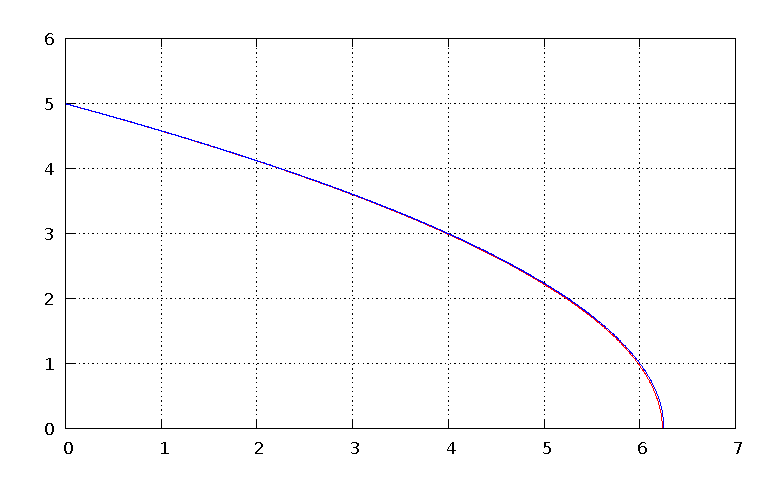
\includegraphics[width=.45\textwidth]
{figures/geometric_pdes/mcf_sphere_radius.ps}
\caption{Average radius of a sphere of initial radius $r_0=5$ subject to
mean curvature flow. In blue the analytical solution while in red the computed
one.}
\label{fig:mcf_sphere_radius}
\end{figure}

\subsection[Equidistribution property]{Equidistribution property}
Finally, we need to introduce a mass lumped inner product on $\Gamma^m$, that
is crucial for the desired tangential motion of vertices on $\Gamma^m$. This
induced tangential motion will lead to good interface mesh properties.

The number of mesh elements is $J_\Gamma=32$.

\begin{figure}[htbp]
\centering
\subfloat[$t=0$]{
\includegraphics[width=.45\textwidth]{figures/geometric_pdes/sd_circle_0.ps}}
\quad
\subfloat[$t=0.05$]{
\includegraphics[width=.45\textwidth]{figures/geometric_pdes/sd_circle_005.ps}}
\\
\subfloat[$t=0.25$]{
\includegraphics[width=.45\textwidth]{figures/geometric_pdes/sd_circle_025.ps}}
\quad
\subfloat[$t=10$]{
\includegraphics[width=.45\textwidth]{figures/geometric_pdes/sd_circle_10.ps}}
\caption{Surface evolution of a circle of initial radius $r_0=0.5$ subject to
surface diffusion.}
\label{fig:sd_circle}
\end{figure}

\begin{figure}[htbp]
\centering
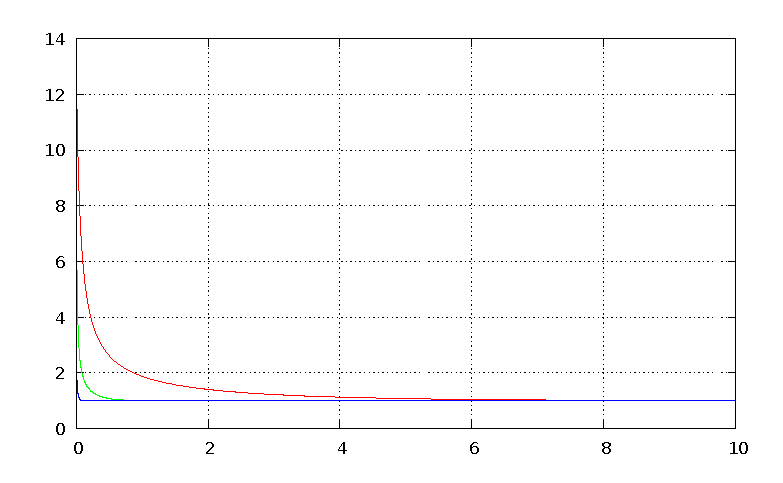
\includegraphics[width=.45\textwidth]
{figures/geometric_pdes/sd_circle_tau.ps}
\caption{Time evolution of the ratio
$\frac{\max_{\sigma\in \Gamma^m}(\surfvol(\sigma))}
{\min_{\sigma\in\Gamma^m}(\surfvol(\sigma))}$ for a circle of initial radius
$r_0=0.5$ subject to surface diffusion. In red $\tau=10^{-2}$, in green
$\tau=10^{-3}$ and in blue $\tau=10^{-4}$.}
\label{fig:sd_circle_tau}
\end{figure}

\chapter{\sc Chapter 2}
\label{ch:2}

\section[Section 1]{Section 1}
\chapter{\sc Chapter 3}
\label{ch:3}

\section[Section 1]{Section 1}
\chapter{\sc Arbitrary Lagrangian Eulerian method}
\label{ch:4}

\section[Section 1]{Section 1}
\chapter{\sc Conclusion}\label{ch:conclusion}

In this thesis we have investigated fitted front tracking finite element
methods for two-phase incompressible Navier--Stokes flows. In Chapter
\ref{ch:introduction}, after introducing the free-boundary fluid flows, we have
described the Navier--Stokes equations which model the evolution of a two-phase
fluid. In these types of problems, apart from the flow solution in the bulk
domain, the interface dividing the phases needs to be determined. Therefore, we
have briefly overviewed the different ways to treat the unknown interface and we
have detailed the various numerical challenges posed by these types of flows.
In Chapter \ref{ch:geometric_pdes} we have introduced the key ideas of the
front tracking approach, applying it to the simple problem of purely geometric
evolution equations such as mean curvature flow and surface diffusion. Here we
have reported on the finite element approximations and we have performed some
numerical experiments in order to show the property of the schemes and of the
flows. In particular, we have shown that the mesh naturally equidistributes and
that the volume is conserved. In Chapter \ref{ch:stokes} we have proposed a
novel finite element approximation for incompressible two-phase Stokes flow.
After showing an energy bound and the volume conservation for the weak problem,
we have demonstrated that our scheme is unconditionally stable and we have
proved the existence and uniqueness of the discrete approximation. Moreover, we
have investigated the equidistribution property and the volume conservation. We
have also discussed the mesh generation process together with the smoothing and
remeshing procedures used to preserve the mesh quality. In Chapter
\ref{ch:stokes_results} we have presented several numerical experiments in 2d
and 3d to test our method and to allow comparisons with other methods. Using
two exact solutions to the two-phase Stokes flow, we have performed various
convergence tests. Moreover, we have tested that interface mesh points are
naturally equidistributed by our scheme, that our scheme conserves the enclosed
volume and that the surface energy monotonically decays. We have also reported
on a shear flow experiment. In Chapter \ref{ch:navier_stokes} we have extended
our Stokes scheme to solve the incompressible two-phase Navier--Stokes flow.
Here, we have derived a standard finite element approximation and an alternative
finite element approximation based on an antisymmetric rewrite. For the
antisymmetric discretization, we have proved the existence and uniqueness of a
discrete solution and we have demonstrated that this scheme has certain
stability properties. We have also examined the techniques used to interpolate
the velocity. In Chapter \ref{ch:ale} we have presented a different finite
element approximation for incompressible two-phase Navier--Stokes flow, which
uses the Arbitrary Lagrangian Eulerian method. This technique allows to
rewrite the velocity time derivative with respect to a fixed reference
manifold. As a consequence, the velocity does not need to be interpolated
anymore. Finally, in Chapter \ref{ch:ns_results} we have tested our schemes in
several numerical experiments. Using two exact solutions to the two-phase
Navier--Stokes flow, we have performed various convergence tests. Then, we have
reported on two rising bubble experiments which constitute the standard
benchmark for two-phase schemes. Here, we have observed that both the ALE and
the standard scheme perform extremely well in terms of accuracy and CPU time.
Moreover, in the case of non-convex bulk domains, we have noticed that the
standard scheme is much slower than the ALE scheme since an unoptimized velocity
interpolation routine has to be used.

There are several lines of research arising from this thesis which should be
investigated in order to further improve the accuracy and the performance of
the schemes presented. The main ones can be summarized as follows:
\begin{itemize}
\item higher order time discretization schemes;
\item solvers and preconditioners for the algebraic linear systems;
\item adaptive bulk mesh refinement and coarsening algorithms;
\item mesh smoothing techniques;
\item higher order spaces for the interface displacement and curvilinear
bulk meshes.
\end{itemize}

\begin{appendices}
\chapter{Some proofs}\label{ch:appx}
In this appendix we report all the passages missing in Sec.(\ref{sec:grad_shavranov}) to arrive at the Grad-Shavranov equation.

\section{Divergence of the pressure tensor}
Derivation of Eq.(\ref{eq:div_press}).
\begin{equation*}
  \begin{split}
    \nabla\cdot\mathbb{P}&=\nabla\cdot[p_\perp \mathbb{I} + ( p_\parallel - p_\perp ) \mathbf{b}\mathbf{b}]=
    \nabla\cdot(p_\perp \mathbb{I}) + \nabla\cdot[( p_\parallel - p_\perp ) \mathbf{b}\mathbf{b}]=\\
    &=\nabla p_\perp+(p_\parallel-p_\perp)\nabla\cdot(\mathbf{b}\mathbf{b})+\mathbf{b}\mathbf{b}\cdot\nabla(p_\parallel-p_\perp)=\\
    &=\nabla p_\perp+(p_\parallel-p_\perp)\nabla\cdot(\mathbf{b}\mathbf{b})+\mathbf{b}\big(\mathbf{b}\cdot\nabla(p_\parallel-p_\perp)\big)=\\
    &=\nabla p_\perp+(p_\parallel-p_\perp)[(\nabla\cdot\mathbf{b})\mathbf{b}+(\mathbf{b}\cdot\nabla)\mathbf{b}]+\big(\mathbf{b}\cdot\nabla(p_\parallel-p_\perp)\big)\mathbf{b}=\\
    &=\nabla p_\perp+(p_\parallel-p_\perp)\Big[\big(\nabla\cdot(B^{-1}\mathbf{B})\big)\mathbf{b}+\mathbf{k}\Big]+\big(\mathbf{b}\cdot\nabla(p_\parallel-p_\perp)\big)\mathbf{b}=\\
    &=\nabla p_\perp+(p_\parallel-p_\perp)\Big\{\big[\nabla B^{-1}\cdot\mathbf{B}+B^{-1}(\nabla\cdot\mathbf{B})\big]\mathbf{b}+\mathbf{k}\Big\}+\big(\mathbf{b}\cdot\nabla(p_\parallel-p_\perp)\big)\mathbf{b}=\\
    &\overset{\mbox{(\ref{eq:MHD_maxwell})}}{=}\nabla p_\perp+(p_\parallel-p_\perp)\Big\{\big[\nabla B^{-1}\cdot\mathbf{B}\big]\mathbf{b}+\mathbf{k}\Big\}+\big(\mathbf{b}\cdot\nabla(p_\parallel-p_\perp)\big)\mathbf{b}=\\
    &=\nabla p_\perp+(p_\parallel-p_\perp)\Big[\big( -B^{-2}\nabla B\cdot\mathbf{B}\big)\mathbf{b}+\mathbf{k}\Big]+\big(\mathbf{b}\cdot\nabla(p_\parallel-p_\perp)\big)\mathbf{b}=\\
    &=\nabla p_\perp+(p_\parallel-p_\perp)\Big[\big( -B^{-1}\nabla B\cdot\mathbf{b}\big)\mathbf{b}+\mathbf{k}\Big]+\big(\mathbf{b}\cdot\nabla(p_\parallel-p_\perp)\big)\mathbf{b}=\\
    &=\nabla p_\perp+(p_\parallel-p_\perp)\Big[ -B^{-1}\big(\nabla B\cdot\mathbf{b}\big)\mathbf{b}+\mathbf{k}\Big]+\big(\mathbf{b}\cdot\nabla(p_\parallel-p_\perp)\big)\mathbf{b}=\\
    &=\nabla p_\perp+(p_\parallel-p_\perp)\mathbf{k}+\Big[\mathbf{b}\cdot\nabla(p_\parallel-p_\perp)-B^{-1}(p_\parallel-p_\perp)\nabla B\cdot\mathbf{b}\Big]\mathbf{b}.
 \end{split}
\end{equation*}

\section{Pressure balance equation}
Derivation of Eq.(\ref{eq:pressure_balance}).
\medskip

It holds that
\begin{equation*}
  \mathbf{b} \cdot(\nabla\cdot\mathbb{P})=B^{-1}\mathbf{B}\cdot(\nabla\cdot\mathbb{P})\overset{\mbox{(\ref{eq:MHD_momentum})}}{=} B^{-1}\mathbf{B}\cdot(\nabla\times\mathbf{B})\times\mathbf{B}=B^{-1}(\nabla\times\mathbf{B})\cdot\mathbf{B}\times\mathbf{B}=0
\end{equation*}
and
\begin{equation*}
  \begin{split}
    \mathbf{b} \cdot(\nabla\cdot\mathbb{P}) &\overset{\mbox{(\ref{eq:div_press})}}{=}
    \mathbf{b}\cdot\bigg\{\nabla p_\perp+(p_\parallel-p_\perp)\mathbf{k}+\Big[\mathbf{b}\cdot\nabla(p_\parallel-p_\perp)-B^{-1}(p_\parallel-p_\perp)\nabla B\cdot\mathbf{b}\Big]\mathbf{b}\bigg\}=\\
    &=\mathbf{b}\cdot\nabla p_\perp+(p_\parallel-p_\perp)\mathbf{k}\cdot\mathbf{b}+\Big[\mathbf{b}\cdot\nabla(p_\parallel-p_\perp)-B^{-1}(p_\parallel-p_\perp)\nabla B\cdot\mathbf{b}\Big]\mathbf{b}\cdot\mathbf{b}=\\
    &=\mathbf{b}\cdot\nabla p_\perp+(p_\parallel-p_\perp)\mathbf{k}\cdot\mathbf{b}+\Big[\mathbf{b}\cdot\nabla(p_\parallel-p_\perp)-B^{-1}(p_\parallel-p_\perp)\nabla B\cdot\mathbf{b}\Big]B^{-2}\mathbf{B}\cdot\mathbf{B}=\\
    &=\mathbf{b}\cdot\nabla p_\perp+(p_\parallel-p_\perp)\mathbf{k}\cdot\mathbf{b}+\mathbf{b}\cdot\nabla(p_\parallel-p_\perp)-B^{-1}(p_\parallel-p_\perp)\nabla B\cdot\mathbf{b}=\\
    &=\mathbf{b}\cdot[\nabla p_\perp+\nabla(p_\parallel-p_\perp)]+(p_\parallel-p_\perp)\mathbf{k}\cdot\mathbf{b}-B^{-1}(p_\parallel-p_\perp)\nabla B\cdot\mathbf{b}=\\
    &=\mathbf{b}\cdot\nabla p_\parallel+(p_\parallel-p_\perp)\mathbf{k}\cdot\mathbf{b}-B^{-1}(p_\parallel-p_\perp)\nabla B\cdot\mathbf{b}=\\
    &\overset{\mbox{(\ref{eq:kb0})}}{=}\mathbf{b}\cdot\nabla p_\parallel-B^{-1}(p_\parallel-p_\perp)\nabla B\cdot\mathbf{b}=\\
    &=\mathbf{b}\cdot\nabla p_\parallel-B^{-1}(p_\parallel-p_\perp)\mathbf{b}\cdot\nabla B=\\
    &=(\mathbf{b}\cdot\nabla) p_\parallel-B^{-1}(p_\parallel-p_\perp)(\mathbf{b}\cdot\nabla) B=\\
    &=\frac{\partial p_\parallel}{\partial l} -B^{-1}(p_\parallel-p_\perp)\frac{\partial B}{\partial l}
  \end{split}
\end{equation*}
where $l$ is the arc length of $\mathbf{B}$ that increase in which $\mathbf{B}$ points, so $l$ measures the distance along the magnetic field-line, and
\begin{equation}\label{eq:kb0}
  \begin{split}
    \mathbf{k}\cdot\mathbf{b}&=(\mathbf{b}\cdot\nabla)\mathbf{b}\cdot\mathbf{b}=\sum_i(\sum_j b_j \frac{\partial b_i}{\partial x_j})b_i=\sum_i\sum_j b_j \frac{\partial b_i}{\partial x_j}b_i=\\
    &=\sum_i\sum_j b_j \frac{\partial}{\partial x_j}(b_i^2/2)=\sum_j b_j \frac{\partial}{\partial x_j}(\frac{1}{2}\sum_i b_i^2)=\\
    &=\frac{1}{2}\sum_j b_j \frac{\partial}{\partial x_j}(\sum_i b_i^2)=(\mathbf{b}\cdot\nabla)(\mathbf{b}\cdot\mathbf{b})/2=(\mathbf{b}\cdot\nabla)(1/2)=0.
  \end{split}
\end{equation}
Then the longitudinal pressure balance equation states that only if $p_\perp>p_\parallel$ it is possible to balance the plasma pressure $p_\parallel$ by means of a positive gradient of $\mathbf{B}$:
\begin{equation}
 \frac{\partial p_\parallel}{\partial l}=B^{-1}(p_\parallel-p_\perp)\frac{\partial B}{\partial l}\quad\Rightarrow\quad B\frac{\partial p_\parallel}{\partial l}\frac{\partial l}{\partial B}=p_\parallel-p_\perp
\end{equation}
that is
\begin{equation*}
  B\frac{\partial p_\parallel}{\partial B}=p_\parallel-p_\perp\quad\Rightarrow\quad p_\perp=p_\parallel-B\frac{\partial p_\parallel}{\partial B}.
\end{equation*}

\section{Magnetic field in covariant basis}
Derivation of Eq.(\ref{eq:covariantB}).
\medskip

The covariant basis is defined as
\begin{equation*}
  \mathbf{e}_i=\mathcal{J} \mathbf{e}^j\times\mathbf{e}^k=\mathcal{J} \nabla j\times\nabla k
\end{equation*}
with the jacobian $\mathcal{J}^{-1}=\nabla r \cdot(\nabla\theta\times\nabla z)=1/r$. Noting that
\begin{equation*}
  \nabla\psi=\frac{\partial\psi}{\partial r}\nabla r+\frac{\partial\psi}{\partial z}\nabla z
\end{equation*}
we have
\begin{equation*}
 \begin{split}
    \mathbf{B}&=\sum_i(\mathbf{B}\cdot\mathbf{e}^i)\mathbf{e}_i=(\mathbf{B}\cdot\nabla r)\mathbf{e}_r+(\mathbf{B}\cdot\nabla\theta)\mathbf{e}_\theta+(\mathbf{B}\cdot\nabla z)\mathbf{e}_z=\\
    &=(\mathbf{B}\cdot\nabla r)\mathbf{e}_r+(\mathbf{B}\cdot\nabla z)\mathbf{e}_z=\\
    &=\left[\frac{\partial\psi}{\partial r}(\nabla r \times\nabla\theta)\cdot\nabla r+\frac{\partial\psi}{\partial z}(\nabla z\times\nabla\theta)\cdot\nabla r\right]\mathbf{e}_r\\
    &+\left[\frac{\partial\psi}{\partial r}(\nabla r \times\nabla\theta)\cdot\nabla z+\frac{\partial\psi}{\partial z}(\nabla z\times\nabla\theta)\cdot\nabla z\right]\mathbf{e}_z=\\
    &=\left[\frac{\partial\psi}{\partial z}(\nabla z\times\nabla\theta)\cdot\nabla r\right]\mathbf{e}_r+\left[\frac{\partial\psi}{\partial r}(\nabla r \times\nabla\theta)\cdot\nabla z\right]\mathbf{e}_z=\\
    &=-\frac{\partial\psi}{\partial z}\nabla r\cdot(\nabla \theta\times\nabla z)\mathbf{e}_r+\frac{\partial\psi}{\partial r}\nabla r\cdot(\nabla \theta\times\nabla z)\mathbf{e}_z=\\
    &=\nabla r\cdot(\nabla \theta\times\nabla z)\left[-\frac{\partial\psi}{\partial z}\mathbf{e}_r+\frac{\partial\psi}{\partial r}\mathbf{e}_z\right]=\\
    &=\mathcal{J}^{-1}\left[-\frac{\partial\psi}{\partial z}\mathbf{e}_r+\frac{\partial\psi}{\partial r}\mathbf{e}_z\right]=\frac{1}{r}\left[-\frac{\partial\psi}{\partial z}\mathbf{e}_r+\frac{\partial\psi}{\partial r}\mathbf{e}_z\right]=\\
    &=-\frac{1}{r}\frac{\partial\psi}{\partial z}\mathbf{e}_r+\frac{1}{r}\frac{\partial\psi}{\partial r}\mathbf{e}_z=B^r\mathbf{e}_r+B^z\mathbf{e}_z\\
  \end{split}
\end{equation*}
so
\begin{equation*}
  B^r=-\frac{1}{r}\frac{\partial\psi}{\partial z},\qquad B^z=\frac{1}{r}\frac{\partial\psi}{\partial r}.
\end{equation*}

\section{Plasma current}
Derivation of Eq.(\ref{eq:plasma_current}).
\medskip

From Eq.(\ref{eq:MHD_momentum}) we have
\begin{equation*}
  \mathbf{B}\times\mathbf{J}\times\mathbf{B}=\mathbf{B}\times\nabla\cdot\mathbb{P}
\end{equation*}
but
\begin{equation*}
  \mathbf{B}\times\mathbf{J}\times\mathbf{B}=(\mathbf{B}\cdot\mathbf{B})\mathbf{J}-(\mathbf{B}\cdot\mathbf{J})\mathbf{B}=B^2\mathbf{J}-(\mathbf{B}\cdot\mathbf{J})\mathbf{B}
\end{equation*}
so
\begin{equation*}
  \mathbf{J}=\frac{1}{B^2}(\mathbf{B}\cdot\mathbf{J})\mathbf{B}+\frac{1}{B^2}\mathbf{B}\times\nabla\cdot\mathbb{P}=(\mathbf{b}\cdot\mathbf{J})\mathbf{b}+\frac{1}{B}\mathbf{b}\times\nabla\cdot\mathbb{P}=J_\parallel\mathbf{b}+\mathbf{J}_\perp.
\end{equation*}
Since
\begin{equation*}
  \begin{split}
    \mathbf{b}\times\nabla\cdot\mathbb{P}&=\mathbf{b}\times\bigg\{\nabla p_\perp+(p_\parallel-p_\perp)\mathbf{k}+\Big[\mathbf{b}\cdot\nabla(p_\parallel-p_\perp)-B^{-1}(p_\parallel-p_\perp)\nabla B\cdot\mathbf{b}\Big]\mathbf{b}\bigg\}=\\
    &=\mathbf{b}\times\big\{\nabla p_\perp+(p_\parallel-p_\perp)\mathbf{k}\big\}=\mathbf{b}\times\nabla p_\perp+(p_\parallel-p_\perp)\mathbf{b}\times\mathbf{k}=\\
    &=\mathbf{b}\times\nabla p_\perp+(p_\parallel-p_\perp)\mathbf{b}\times(\nabla\times\mathbf{b}\times\mathbf{b})=\\
    &=\mathbf{b}\times\nabla p_\perp+(p_\parallel-p_\perp)[(\mathbf{b}\cdot\mathbf{b})\nabla\times\mathbf{b}-(\mathbf{b}\cdot\nabla\times\mathbf{b})\mathbf{b}]=\\
    &=\mathbf{b}\times\nabla p_\perp+(p_\parallel-p_\perp)[\nabla\times\mathbf{b}-(\mathbf{b}\cdot\nabla\times\mathbf{b})\mathbf{b}]=\\
    &=\mathbf{b}\times\nabla p_\perp+(p_\parallel-p_\perp)[B^{-1}\nabla\times\mathbf{B}+\nabla(B^{-1})\times\mathbf{B}-(\mathbf{b}\cdot\nabla\times\mathbf{b})\mathbf{b}]=\\
    &=\mathbf{b}\times\nabla p_\perp+B^{-1}(p_\parallel-p_\perp)[\nabla\times\mathbf{B}-B^{-1}\nabla B\times\mathbf{B}-(\mathbf{b}\cdot B\nabla\times\mathbf{b})\mathbf{b}]=\\
    &=\mathbf{b}\times\nabla p_\perp+B^{-1}(p_\parallel-p_\perp)[\mathbf{J}-\nabla B\times\mathbf{b} -(\mathbf{b}\cdot (\nabla\times\mathbf{B}-\nabla B\times\mathbf{b})\mathbf{b}]=\\
    &=\mathbf{b}\times\nabla p_\perp+B^{-1}(p_\parallel-p_\perp)[\mathbf{J}-\nabla B\times\mathbf{b} -(\mathbf{b}\cdot (\mathbf{J}-\nabla B\times\mathbf{b})\mathbf{b}]=\\
    &=\mathbf{b}\times\nabla p_\perp+B^{-1}(p_\parallel-p_\perp)[\mathbf{J}-\nabla B\times\mathbf{b} -(\mathbf{b}\cdot\mathbf{J})\mathbf{b}-(\mathbf{b}\cdot\nabla B\times\mathbf{b})\mathbf{b}]=\\
    &=\mathbf{b}\times\nabla p_\perp+B^{-1}(p_\parallel-p_\perp)[\mathbf{J}-(\mathbf{b}\cdot\mathbf{J})\mathbf{b}-\nabla B\times\mathbf{b}]=\\
    &=\mathbf{b}\times\nabla p_\perp+B^{-1}(p_\parallel-p_\perp)[\mathbf{J}_\perp+\mathbf{b}\times\nabla B]=\\
    &=\mathbf{b}\times[\nabla p_\perp+B^{-1}(p_\parallel-p_\perp)\nabla B]+B^{-1}(p_\parallel-p_\perp)\mathbf{J}_\perp=\\
    &=\mathbf{b}\times[\nabla p_\perp-B^{-1}(p_\perp-p_\parallel)\nabla B]-B^{-1}(p_\perp-p_\parallel)\mathbf{J}_\perp\\
  \end{split}
\end{equation*}
we have
\begin{equation*}
  \begin{split}
    \mathbf{J}_\perp&=B^{-1}\mathbf{b}\times\nabla\cdot\mathbb{P}= B^{-1}\mathbf{b}\times[\nabla p_\perp-B^{-1}(p_\perp-p_\parallel)\nabla B]-B^{-2}(p_\perp-p_\parallel)\mathbf{J}_\perp=\\\
    &=\mathbf{b}\times[B^{-1}\nabla p_\perp-B^{-2}(p_\perp-p_\parallel)\nabla B]-B^{-2}(p_\perp-p_\parallel)\mathbf{J}_\perp=\\
    &=\mathbf{b}\times[B^{-1}\nabla p_\perp-\eta\nabla B]-\eta\mathbf{J}_\perp\\
  \end{split}
\end{equation*}
where $\eta=B^{-2}(p_\perp-p_\parallel)$. Then
\begin{equation*}
  \begin{split}
    (1+\eta)\mathbf{J}_\perp&=\mathbf{b}\times[B^{-1}\nabla p_\perp-\eta\nabla B]=\\
    &=\mathbf{b}\times[B^{-1}\nabla p_\perp-B^{-1}\nabla p_\parallel+B^{-1}\nabla p_\parallel-\eta\nabla B]=\\
    &=\mathbf{b}\times[B^{-1}(\nabla p_\perp-\nabla p_\parallel)+B^{-1}\nabla p_\parallel-\eta\nabla B]=\\
    &=\mathbf{b}\times[B^{-1}\nabla( p_\perp- p_\parallel)+B^{-1}\nabla p_\parallel-\eta\nabla B]=\\
    &=\mathbf{b}\times[\nabla\big(B^{-1}(p_\perp- p_\parallel)\big)-(p_\perp- p_\parallel)\nabla B^{-1}+B^{-1}\nabla p_\parallel-\eta\nabla B]=\\
    &=\mathbf{b}\times[\nabla\big(B^{-1}(p_\perp- p_\parallel)\big)+B^{-2}(p_\perp- p_\parallel)\nabla B+B^{-1}\nabla p_\parallel-\eta\nabla B]=\\
    &=\mathbf{b}\times[\nabla\big(BB^{-2}(p_\perp- p_\parallel)\big)+\eta\nabla B+B^{-1}\nabla p_\parallel-\eta\nabla B]=\\
    &=\mathbf{b}\times[\nabla(\eta B)+B^{-1}\nabla p_\parallel]=\\
    &=\mathbf{b}\times[B\nabla\eta+\eta\nabla B+B^{-1}\nabla p_\parallel].\\
  \end{split}
\end{equation*}
Using the fact that
\begin{equation*}
  \nabla p_\parallel=\frac{\partial p_\parallel}{\partial \psi}\nabla\psi+\frac{\partial p_\parallel}{\partial B}\nabla B \overset{\mbox{(\ref{eq:pressure_balance})}}{=}
  \frac{\partial p_\parallel}{\partial \psi}\nabla\psi+B^{-1}(p_\parallel-p_\perp)\nabla B
\end{equation*}
we find
\begin{equation*}
  \begin{split}
    (1+\eta)\mathbf{J}_\perp&=\mathbf{b}\times\left[B\nabla\eta+\eta\nabla B+B^{-1}\left(\frac{\partial p_\parallel}{\partial \psi}\nabla\psi+B^{-1}(p_\parallel-p_\perp)\nabla B\right)\right]=\\
    &=\mathbf{b}\times\left[B\nabla\eta+\eta\nabla B+B^{-1}\frac{\partial p_\parallel}{\partial \psi}\nabla\psi-B^{-2}(p_\perp-p_\parallel)\nabla B\right]=\\
    &=\mathbf{b}\times\left[B\nabla\eta+\eta\nabla B+B^{-1}\frac{\partial p_\parallel}{\partial \psi}\nabla\psi-\eta\nabla B\right]=\\
    &=\mathbf{b}\times\left[B\nabla\eta+B^{-1}\frac{\partial p_\parallel}{\partial \psi}\nabla\psi\right]=\\
    &=\mathbf{B}\times\nabla\eta+B^{-2}\frac{\partial p_\parallel}{\partial \psi}\mathbf{B}\times\nabla\psi.
  \end{split}
\end{equation*}
So
\begin{equation*}
  \mathbf{J}_\perp=\frac{1}{1+\eta}\left[\mathbf{B}\times\nabla\eta+B^{-2}\frac{\partial p_\parallel}{\partial \psi}\mathbf{B}\times\nabla\psi\right]
\end{equation*}
From the Clebsch representation of magnetic field and for the independence of any function from the poloidal angle we have:
\begin{enumerate}
 \item $\mathbf{B}\times\nabla\eta=(\nabla\psi\times\nabla\theta)\times\nabla\eta=(\nabla\eta\cdot\nabla\psi)\nabla\theta-(\nabla\eta\cdot\nabla\theta)\nabla\psi=(\nabla\eta\cdot\nabla\psi)\nabla\theta$
  \item $\mathbf{B}\times\nabla\psi=(\nabla\psi\times\nabla\theta)\times\nabla\psi=(\nabla\psi\cdot\nabla\psi)\nabla\theta=|\nabla\psi|^2\nabla\theta$
\end{enumerate}
and from the covariant basis $(\mathbf{e}_r,\mathbf{e}_\theta,\mathbf{e}_z)$
\begin{equation*}
  B^2=|\mathbf{B}|^2=|-\frac{1}{r}\frac{\partial\psi}{\partial z}\mathbf{e}_r+\frac{1}{r}\frac{\partial\psi}{\partial r}\mathbf{e}_z|^2=\frac{1}{r^2}[(\frac{\partial\psi}{\partial z})^2+(\frac{\partial\psi}{\partial r})^2]=\frac{|\nabla\psi|^2}{r^2}
\end{equation*}
so that $\mathbf{B}\times\nabla\psi=r^2 B^2\nabla\theta$ then
\begin{equation*}
  \mathbf{J}_\perp=\frac{1}{1+\eta}\left[(\nabla\eta\cdot\nabla\psi)+r^2\frac{\partial p_\parallel}{\partial \psi}\right]\nabla\theta.
\end{equation*}

\section{Grad-Shafranov equation}
Derivation of Eq.(\ref{eq:GS_eq}).
\medskip

For hypothesis $\partial_\theta=0$ and we notice that $B^\theta=0$ so
\begin{equation*}
  \nabla\times\mathbf{B}=\displaystyle
    \begin{vmatrix}
      \displaystyle\frac{1}{r}\mathbf{e}_r & \mathbf{e}_\theta & \displaystyle\frac{1}{r}\mathbf{e}_z\\
      \partial_r & 0 & \partial_z\\
    B^r & 0 & B^z
  \end{vmatrix}
  =\left[\partial_z\left(-\frac{1}{r}\frac{\partial\psi}{\partial z}\right)-\partial_r\left(\frac{1}{r}\frac{\partial\psi}{\partial r}\right)\right]\mathbf{e}_\theta.
\end{equation*}
Then for Eq.(\ref{eq:MHD_current}) we know that
\begin{equation*}
  \mathbf{J}=-\left[\frac{\partial}{\partial z}\left(\frac{1}{r}\frac{\partial\psi}{\partial z}\right)+\frac{\partial}{\partial r}\left(\frac{1}{r}\frac{\partial\psi}{\partial r}\right)\right]\mathbf{e}_\theta
  =-\left[\frac{\partial}{\partial r}\left(\frac{1}{r}\frac{\partial\psi}{\partial r}\right)+\frac{1}{r}\frac{\partial^2\psi}{\partial z^2}\right]\mathbf{e}_\theta=J^\theta\mathbf{e}_\theta
\end{equation*}
therefore
\begin{equation*}
  J_\parallel=B^{-1}\mathbf{J}\cdot\mathbf{B}=B^{-1}[J^\theta\mathbf{e}_\theta\cdot(B^r\mathbf{e}_r+B^z\mathbf{e}_z)]=0.
\end{equation*}
So we have that $\mathbf{J}\equiv\mathbf{J}_\perp$, that is
\begin{equation*}
  -\left[\frac{\partial}{\partial r}\left(\frac{1}{r}\frac{\partial\psi}{\partial r}\right)+\frac{1}{r}\frac{\partial^2\psi}{\partial z^2}\right]\mathbf{e}_\theta
  =\frac{1}{1+\eta}\left[(\nabla\eta\cdot\nabla\psi)+r^2\frac{\partial p_\parallel}{\partial \psi}\right]\nabla\theta.
\end{equation*}
As $\mathbf{e}_\theta=r\nabla\theta$, then
\begin{equation*}
 -\left[r\frac{\partial}{\partial r}\left(\frac{1}{r}\frac{\partial\psi}{\partial r}\right)+\frac{\partial^2\psi}{\partial z^2}\right]
=\frac{1}{1+\eta}\left[(\nabla\eta\cdot\nabla\psi)+r^2\frac{\partial p_\parallel}{\partial \psi}\right]
\end{equation*}
or
\begin{equation*}
  -\Delta^*\psi=\frac{1}{1+\eta}\left[(\nabla\eta\cdot\nabla\psi)+r^2\frac{\partial p_\parallel}{\partial \psi}\right].
\end{equation*}
As $\eta=B^{-2}(p_\perp-p_\parallel)$ and from (\ref{eq:pressure_balance}) it results $B^{-1}(p_\perp-p_\parallel)=-\partial_B p_\parallel$, this means that
\begin{equation*}
  \eta=-B^{-1}\frac{\partial p_\parallel}{\partial B}
\end{equation*}
then
\begin{equation*}
  -\Delta^*\psi=\frac{1}{1-B^{-1}\partial_B p_\parallel}\left[-\nabla(B^{-1}\partial_B p_\parallel)\cdot\nabla\psi+r^2\partial_\psi p_\parallel\right].
\end{equation*}
Focusing on the definition of Grad-Shafranov operator we can notice that
\begin{equation*}
  \begin{split}
    \Delta^*\psi&=r\left[\frac{\partial}{\partial r}\left(\frac{1}{r}\frac{\partial\psi}{\partial r}\right)+\frac{1}{r}\frac{\partial^2\psi}{\partial z^2}\right]=r\frac{\partial}{\partial r}\left(\frac{1}{r}\frac{\partial\psi}{\partial r}\right)+\frac{\partial^2\psi}{\partial z^2}=r^2\nabla\cdot\left(\frac{1}{r^2}\nabla\psi\right)=\\
    &=-\frac{1}{r}\frac{\partial\psi}{\partial r}+\frac{\partial^2\psi}{\partial r^2}+\frac{\partial^2\psi}{\partial z^2}=\frac{1}{r}\frac{\partial\psi}{\partial r}+\frac{\partial^2\psi}{\partial r^2}+\frac{\partial^2\psi}{\partial z^2}-\frac{2}{r}\frac{\partial\psi}{\partial r}=\Delta\psi-\frac{2}{r}\frac{\partial\psi}{\partial r}
  \end{split}
\end{equation*}
so
\begin{equation*}
 \Delta^*\psi=r^2\nabla\cdot\left(\frac{1}{r^2}\nabla\psi\right)=\Delta\psi-\frac{2}{r}\frac{\partial\psi}{\partial r}.
\end{equation*}

\end{appendices}

\setstretch{1.2}

\clearpage
\bibliographystyle{siam}
\bibliography{../bib/robert_refs,../bib/marco_refs}
%{\def\bysame{\leavevmode\hbox 
to3em{\hrulefill}\thinspace}\newcommand{\NUMBERRRR}{\#}\newcommand{\PAGESS}{}
\phantomsection\addcontentsline{toc}{chapter}{References}
\begin{thebibliography}{99}
\bibitem{1} Name, \emph{Title,} Journal {\bf Issue} (Date)\PAGESS{}0--0.
\bibitem{2} \bysame, \emph{Title,} Journal {\bf Issue} (Date) \PAGESS{}0--0.
\end{thebibliography}}

\end{document}
